% CrowdGuard AI - Dissertation (RRU format)
% Compile on Overleaf with pdfLaTeX. Upload this folder (main.tex + images/).
\documentclass[12pt,a4paper,oneside]{report}

\usepackage[utf8]{inputenc}
\usepackage[T1]{fontenc}
\usepackage{newtxtext,newtxmath}          % Times New Roman
\usepackage[a4paper,left=38mm,right=25.4mm,top=25.4mm,bottom=25.4mm]{geometry}
\usepackage{setspace}
\usepackage{graphicx}
\usepackage{booktabs,array,tabularx,multirow}
\usepackage{float}
\usepackage{xcolor}
\usepackage{enumitem}
\usepackage{caption}
\usepackage{titlesec}
\usepackage{tocloft}
\usepackage{fancyhdr}
\usepackage{tikz}
\usetikzlibrary{arrows.meta,positioning}
\usepackage{pgfplots}
\pgfplotsset{compat=1.17}
\usepackage[numbers,super,sort&compress]{natbib}
\usepackage[hidelinks]{hyperref}

\onehalfspacing
\setlength{\parindent}{0pt}
\setlength{\parskip}{6pt}
\captionsetup{font=small,labelfont=bf}
\setlist{itemsep=2pt,topsep=4pt}

% Chapter headings: "Chapter 1" on one line, title below, centred
\titleformat{\chapter}[display]{\normalfont\bfseries\centering}{\Large\chaptertitlename\ \thechapter}{8pt}{\LARGE}
\titlespacing*{\chapter}{0pt}{-10pt}{20pt}
\titleformat{\section}{\normalfont\large\bfseries}{\thesection}{1em}{}
\titleformat{\subsection}{\normalfont\normalsize\bfseries}{\thesubsection}{1em}{}

\renewcommand{\contentsname}{\centering TABLE OF CONTENTS}
\renewcommand{\listfigurename}{\centering List of Figures}
\renewcommand{\listtablename}{\centering List of Tables}
\renewcommand{\bibname}{Bibliography and References}
\renewcommand{\cftchapleader}{\cftdotfill{\cftdotsep}}

\pagestyle{fancy}
\fancyhf{}
\fancyfoot[C]{\thepage}
\renewcommand{\headrulewidth}{0pt}
\fancypagestyle{plain}{\fancyhf{}\fancyfoot[C]{\thepage}\renewcommand{\headrulewidth}{0pt}}

% ---------- details to fill in ----------
\newcommand{\thesistitle}{CROWDGUARD AI: AN INTEGRATED SYSTEM FOR CROWD THREAT MONITORING AND DEEPFAKE MEDIA VERIFICATION}
\newcommand{\degreename}{[Degree Name]}
\newcommand{\studentname}{SAURAV MATHUR}
\newcommand{\enrolment}{[Enrolment No.]}
\newcommand{\supervisor}{[NAME OF SUPERVISOR]}
\newcommand{\supdesignation}{[Designation]}
\newcommand{\schoolname}{[NAME OF THE SCHOOL]}
\newcommand{\submissiondate}{[Month \& Year]}
% ----------------------------------------

\newcommand{\screenshot}[2]{%
  \begin{figure}[H]\centering
  \fbox{\parbox[c][5.5cm][c]{0.85\textwidth}{\centering\small\textit{Insert screenshot here:}\\[4pt] #1}}
  \caption{#1}\label{#2}
  \end{figure}}

\newcommand{\titlepagebody}[1]{%
  \begin{center}
  {\fontsize{16}{20}\selectfont\bfseries \thesistitle\par}
  \vspace{14pt}
  {\fontsize{14}{17}\selectfont Dissertation submitted\par}
  \vspace{4pt}
  {\fontsize{16}{19}\selectfont\bfseries to\par}
  {\fontsize{16}{19}\selectfont\bfseries RASHTRIYA RAKSHA UNIVERSITY\par}
  {\fontsize{12}{15}\selectfont (An Institution of National Importance)\par}
  \vspace{10pt}
  {\fontsize{14}{17}\selectfont For the partial fulfilment for the award of the degree of\par}
  \vspace{6pt}
  {\fontsize{24}{29}\selectfont\bfseries \degreename\par}
  \vspace{12pt}
  {\fontsize{14}{17}\selectfont Submitted by\par}
  {\fontsize{12}{15}\selectfont\bfseries \studentname\par}
  {\fontsize{10}{12}\selectfont\bfseries (\enrolment)\par}
  \vspace{12pt}
  {\fontsize{16}{19}\selectfont\bfseries Under the Guidance of\par}
  {\fontsize{12}{15}\selectfont\bfseries \supervisor\par}
  {\fontsize{12}{15}\selectfont \supdesignation,\par \schoolname,\par Place\par}
  \vspace{12pt}
  \includegraphics[height=3.2cm]{#1}\par
  \vspace{10pt}
  {\fontsize{13}{16}\selectfont\bfseries \schoolname\par}
  {\fontsize{12}{15}\selectfont\bfseries RASHTRIYA RAKSHA UNIVERSITY,\par
   Lavad, Dehgam, Gandhinagar-382305, Gujarat, India\par
   \vspace{6pt}\submissiondate\par}
  \end{center}}

\begin{document}

% ================= FRONT PAGE AND COVER PAGE =================
\begin{titlepage}\titlepagebody{images/image1.png}\end{titlepage}
\begin{titlepage}\titlepagebody{images/image2.png}\end{titlepage}

\pagenumbering{roman}
\setcounter{page}{1}

% ================= DECLARATION =================
\chapter*{\centering DECLARATION}
\addcontentsline{toc}{chapter}{Declaration}
The work embodied in this Dissertation titled ``CrowdGuard AI: An Integrated System for Crowd Threat Monitoring and Deepfake Media Verification'' submitted for the partial fulfillment of the degree of \degreename{} is the original research work carried out by me. The research work does not form the basis for the award of any degree, diploma, associateship, fellowship or other titles in the Rashtriya Raksha University or similar institutions of higher learning. All the ideas and references have been duly acknowledged.

\vspace{2.5cm}
\hfill (Name \& Signature of the Candidate)

\vspace{1cm}
\textbf{Date:}

% ================= CERTIFICATE =================
\chapter*{\centering CERTIFICATE}
\addcontentsline{toc}{chapter}{Certificate}
This is to certify that the Dissertation titled ``CrowdGuard AI: An Integrated System for Crowd Threat Monitoring and Deepfake Media Verification'' was carried out by Mr.\ Saurav Mathur (Enrollment no.\ \enrolment) studying at \schoolname{} for partial fulfillment of \degreename{} degree to be awarded by Rashtriya Raksha University. This research work has been carried out under my guidance and supervision and it is up to my satisfaction. The Dissertation is fit to be considered for evaluation for the degree of \degreename.

\vspace{1cm}
Date:\\
Place:

\vspace{2.5cm}
\begin{tabular}{@{}p{0.48\textwidth}p{0.48\textwidth}@{}}
Signature and Name of Supervisor & \hfill Signature and Name of School Director
\end{tabular}

\vspace{1.5cm}
\begin{center}Round Seal of RRU\end{center}

% ================= ACKNOWLEDGEMENTS =================
\chapter*{\centering Acknowledgements}
\addcontentsline{toc}{chapter}{Acknowledgements}
I would like to thank my supervisor, \supervisor, for the guidance given throughout this project. The suggestion to test the system on footage of real incidents, and not only on clean sample images, changed the direction of the work in a useful way.

I am thankful to the faculty of \schoolname{} for the review sessions, where several weak points of the first version were pointed out. Those comments are the reason the deepfake module was measured again and rebuilt in the later part of the project.

This work depends on models and datasets that other researchers have released openly. I acknowledge the authors of Community Forensics, B-Free, UniversalFakeDetect, GenD, YOLOv8, Defactify, DeepFakeFace, FaceForensics++ and Celeb-DF. Without their public code and data, a project of this size would not have been possible in one semester.

Finally, I thank my family and friends for their patience during the long evenings spent waiting for models to finish running.

\vspace{1cm}
\hfill Saurav Mathur

% ================= TOC / LOF / LOT =================
\tableofcontents
\listoffigures
\addcontentsline{toc}{chapter}{List of Figures}
\listoftables
\addcontentsline{toc}{chapter}{List of Tables}

% ================= ABSTRACT =================
\chapter*{}
\addcontentsline{toc}{chapter}{Abstract}
\vspace{-2.5cm}
\begin{center}
\textbf{Abstract: CrowdGuard AI: An Integrated System for Crowd Threat Monitoring and Deepfake Media Verification}\\[6pt]
Submitted By\\ Saurav Mathur\\[4pt]
Supervised By \supervisor, \supdesignation\\[10pt]
\textbf{Abstract}
\end{center}

\textbf{Objective.} Security control rooms now receive crowd footage from CCTV, phones and social media, and some of it may be synthetic or edited. This work builds one system that analyses the physical scene and also checks whether the media itself is authentic.

\textbf{Work done.} CrowdGuard AI has a FastAPI backend and a Next.js web console. The crowd module uses YOLOv8 with ByteTrack to count and track people, flags fast-moving tracks and computes a risk level. The forensics module combines Community Forensics, B-Free and UniversalFakeDetect for whole-image analysis with the GenD model for faces. Testing showed that the first version performed poorly. The causes were a pixel detector whose weights gave the same output for every image, a generic face classifier, no score calibration and hand-tuned decision rules. These were replaced, and Platt calibration with logistic-regression fusion was fitted on 1,031 labelled public images, each scored as the original file and as a JPEG copy.

\textbf{Results.} On 1,010 held-out image variants, detection of fakes rose from 62\% to 79\% and correct acceptance of real images from 76\% to 96\%. Balanced accuracy rose from 69\% to 88\% (AUC 0.943). False alarms on real faces fell from 43\% to 3\%. DALL-E 3 images (40\% detected) and InsightFace swaps (46\%) remain weak.

\textbf{Conclusions.} Fusion weights measured on labelled data were more reliable than hand-set rules. Quantitative video evaluation and a trained weapon detector are left for the next phase.

\clearpage
\pagenumbering{arabic}
\setcounter{page}{1}

% =====================================================================
\chapter{Introduction}
% =====================================================================

\section{Background}
Video is now the main evidence used during a public-order incident. Control rooms watch CCTV, police units forward phone recordings, and clips spread on social media within minutes of an event. Two separate questions have to be answered about such footage. The first is what is happening in the scene: how many people are present, whether the crowd is growing, whether someone is moving abnormally fast and whether a weapon is visible. The second is whether the footage can be trusted at all.

The second question has become harder in the last few years. Generative adversarial networks\cite{goodfellow2014} and later diffusion models\cite{ho2020,rombach2022} can produce photographs that most people cannot tell apart from camera images. Face-swap tools can replace the identity of a person in an existing video\cite{tolosana2020}. A fabricated clip of a crowd attack or a fake image of an armed person can push responders to the wrong place, or be used to discredit real evidence later.

Most existing tools deal with only one of these two questions. Crowd analytics software assumes the input is genuine, and deepfake detectors are usually separate websites or research scripts that know nothing about the scene. This project brings the two checks together in one workflow.

\section{Problem Statement}
The aim is to design and build a system that takes an image or video of a crowd incident and reports (a) the physical threat picture and (b) whether the media appears to be AI-generated or manipulated, and then combines both into one incident verdict. The deepfake verdict must be measured on labelled data. A detector that looks convincing on a few hand-picked samples is not enough for security use.

\section{Objectives}
\begin{enumerate}
  \item Detect and track people in images and video, estimate crowd density and flag abnormal movement.
  \item Detect whole-image AI generation (diffusion and GAN images) and face manipulation (face swaps).
  \item Combine several published detectors so that one weak model does not decide the verdict.
  \item Calibrate the detector scores and fit the fusion weights on public labelled data, then report accuracy on a held-out split.
  \item Report clearly when a check could not run, without silently returning ``authentic''.
  \item Give explanations an operator can read: per-model scores, Error Level Analysis (ELA) and attention heatmaps.
  \item Provide a web console with separate views for surveillance, forensics and combined investigation.
\end{enumerate}

\section{Scope of the Work}
The project covers still images and recorded video files uploaded through the web console, or fetched from a URL. Live RTSP camera streams, a trained weapon detector, optical-flow crowd analysis and PDF incident reports are planned for the second review and are not part of the results in this report. The deepfake evaluation covers images. A labelled video set was prepared, but its full evaluation is listed as pending work in Chapter~6.

\section{Organisation of the Report}
Chapter~2 reviews previous work on synthetic image detection, face-manipulation detection, calibration and crowd monitoring. Chapter~3 gives the requirements and the system design. Chapter~4 describes the implementation. Chapter~5 explains how the first version was tested, what went wrong, and the results after the pipeline was rebuilt. Chapter~6 gives conclusions and future work. Appendix~A lists abbreviations and Appendix~B gives setup commands and the API reference.

% =====================================================================
\chapter{Literature Review}
% =====================================================================

\section{Generative Media and Deepfakes}
Goodfellow et al.\cite{goodfellow2014} introduced GANs, in which a generator and a discriminator are trained against each other. Denoising diffusion models\cite{ho2020} later gave higher quality and more stable training, and latent diffusion\cite{rombach2022} (the basis of Stable Diffusion) made high-resolution generation possible on ordinary GPUs. Commercial systems such as DALL-E 3 and Midjourney are trained in a similar way, but their details are not public. Tolosana et al.\cite{tolosana2020} group face manipulation into entire face synthesis, identity swap, attribute editing and expression swap. Each type leaves different traces.

\section{Detection of AI-Generated Images}
Wang et al.\cite{wang2020} showed that a ResNet-50 trained on images from a single GAN can detect images from several other GANs, provided strong blur and JPEG augmentation is used during training. Generalisation to diffusion models was weaker. Ojha et al.\cite{ojha2023} (UniversalFakeDetect) kept a CLIP ViT-L/14 encoder\cite{radford2021} frozen and trained only a linear layer on top. Their argument was that a general feature space avoids overfitting to one generator. Tan et al.\cite{tan2024} proposed Neighboring Pixel Relationships (NPR), which looks at the local up-sampling pattern that most generators leave behind.

Two recent works are central to this project. Park and Owens\cite{park2025} built Community Forensics, a training set drawn from thousands of different generators, and showed that diversity of generators matters more than model size. Their released detector is a ViT-S/16\cite{dosovitskiy2021} working at 384 pixels. Guillaro et al.\cite{guillaro2025} argued that many detectors learn dataset bias (image size, JPEG format, content) and not generation artefacts. Their B-Free method trains on fake images made by regenerating real ones through Stable Diffusion, so real and fake versions share the same content. It uses a DINOv2\cite{oquab2024} ViT-B with registers\cite{darcet2024} and is applied at native resolution on 504-pixel crops.

\section{Detection of Face Manipulation}
FaceForensics++\cite{rossler2019} and Celeb-DF\cite{li2020} are the standard face-swap benchmarks. Detectors trained on one benchmark often fail on another. Yermakov et al.\cite{yermakov2026} (GenD) fine-tune only the layer-normalisation parameters of a CLIP ViT-L/14 and add metric learning on a hyperspherical feature space. They report state-of-the-art cross-dataset AUROC over 14 benchmarks. GenD expects a face crop that is 1.3 times the detected face box, which matters for the implementation in Chapter~4. The DeepFakeFace dataset\cite{song2023} contains real IMDB-WIKI faces together with InsightFace swaps, Stable Diffusion inpainting and text-to-image faces, so it tests both swap and generation cases.

\section{Calibration and Combination of Detectors}
Raw outputs of neural networks are often badly calibrated. A score of 0.9 does not mean a 90\% chance of being fake\cite{guo2017}. Platt scaling\cite{platt1999} fits a logistic function on held-out data to turn a raw score into a probability. When several detectors are combined, calibrated log-odds can be added with weights learned by logistic regression. This gives a measured weight to each detector, where hand-set rules rely on guesswork. One aim of this project was to replace manual thresholds with this kind of fitted fusion.

\section{Crowd Monitoring}
Single-stage detectors from the YOLO family are widely used for real-time person detection. YOLOv8\cite{jocher2023} provides pretrained COCO models and built-in tracking. ByteTrack\cite{zhang2022} improves multi-object tracking by also associating low-confidence detections, which helps in dense crowds where people are partly hidden. Light classifiers such as MobileNetV3\cite{howard2019} are suitable for a second-stage weapon check on cropped regions.

\section{Explainability and Provenance}
Error Level Analysis\cite{krawetz2007} re-saves an image as JPEG and shows the difference. Regions edited after the last compression often stand out. The C2PA standard\cite{c2pa} defines signed provenance manifests, and some generators also write prompts or software tags into metadata. Neither method is reliable alone. ELA is easily confused by re-compression, and metadata can be removed. Both are still useful as supporting evidence shown next to the model scores.

\section{Research Gap}
The detectors above are evaluated mostly in isolation, on their own test sets. Systems for operators usually stop at a single model and report its raw score. Crowd analytics and media forensics are rarely combined. This project combines published detectors under one calibration fitted on mixed public data, links the result to a crowd threat engine, and measures the final verdict rather than only the separate models.

% =====================================================================
\chapter{System Requirements and Design}
% =====================================================================

\section{Requirements}
\textbf{Functional requirements}
\begin{itemize}
  \item Accept images (JPEG, PNG, WebP) and videos (MP4, MOV, AVI, MKV, WebM) by upload or URL.
  \item Count and track people, detect fast movement and compute a crowd risk level.
  \item Run deepfake analysis in three modes: \emph{Auto}, \emph{Deepfake (face)} and \emph{AI-Generated (whole image)}.
  \item Combine both analyses into an incident verdict.
  \item Show per-model scores, warnings and heatmaps, and allow the operator to submit feedback.
\end{itemize}

\textbf{Non-functional requirements}
\begin{itemize}
  \item Run on a single laptop GPU with 6 GB of memory.
  \item Return an image result within a few seconds.
  \item Never report ``authentic'' when a required check did not run.
  \item Keep model weights out of version control and document how to obtain them.
\end{itemize}

\section{Hardware and Software}
\begin{table}[H]
\centering
\caption{Hardware and software used}\label{tab:env}
\begin{tabular}{@{}ll@{}}
\toprule
Item & Version / Detail \\
\midrule
GPU & NVIDIA GeForce RTX 4050 Laptop, 6 GB \\
Operating system & Windows 10/11 (x64) [confirm] \\
Python & 3.12.10 \\
PyTorch & 2.5.1 with CUDA 12.1 \\
Transformers / timm & 4.56.2 / 1.0.30 \\
Backend framework & FastAPI with Uvicorn\cite{fastapi} \\
Frontend & Next.js 14.2.15, React 18, Tailwind CSS\cite{nextjs} \\
Detection and tracking & Ultralytics YOLOv8\cite{jocher2023} with ByteTrack \\
Image processing & OpenCV\cite{bradski2000}, Pillow \\
\bottomrule
\end{tabular}
\end{table}

\section{Overall Architecture}
Figure~\ref{fig:arch} shows the main parts. The web console sends requests to the FastAPI backend on port 8000. The backend holds the crowd models and the whole-image deepfake detectors on the GPU. The face model runs as a separate worker process on port 8001, started by the backend. It has its own Python environment because its library versions differ from the main application. If the worker is not available, the backend still answers, but it marks the face check as not done.

\begin{figure}[H]
\centering
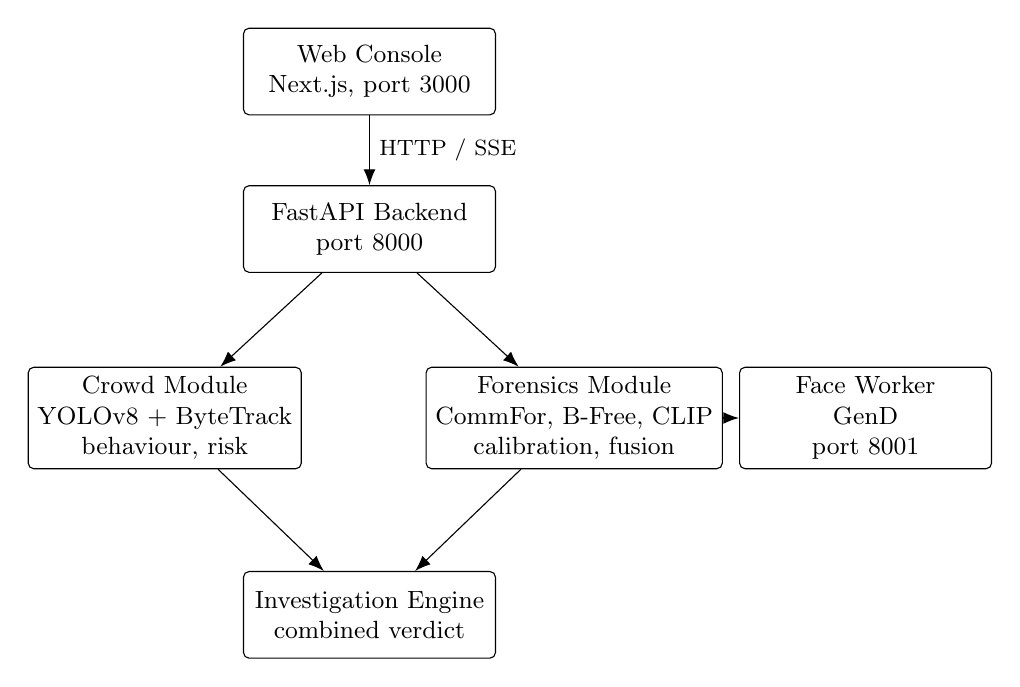
\begin{tikzpicture}[
  box/.style={draw, rounded corners=2pt, align=center, minimum width=32mm, minimum height=11mm, font=\small},
  arr/.style={-{Latex[length=2mm]}}]
\node[box] (ui) at (-1,0) {Web Console\\Next.js, port 3000};
\node[box] (api) at (-1,-2) {FastAPI Backend\\port 8000};
\node[box] (crowd) at (-3.6,-4.4) {Crowd Module\\YOLOv8 + ByteTrack\\behaviour, risk};
\node[box] (foren) at (1.6,-4.4) {Forensics Module\\CommFor, B-Free, CLIP\\calibration, fusion};
\node[box] (gend) at (5.3,-4.4) {Face Worker\\GenD\\port 8001};
\node[box] (inv) at (-1,-6.9) {Investigation Engine\\combined verdict};
\draw[arr] (ui) -- node[right,font=\footnotesize]{HTTP / SSE} (api);
\draw[arr] (api) -- (crowd);
\draw[arr] (api) -- (foren);
\draw[arr] (foren) -- (gend);
\draw[arr] (crowd) -- (inv);
\draw[arr] (foren) -- (inv);
\end{tikzpicture}
\caption{Overall architecture of CrowdGuard AI}\label{fig:arch}
\end{figure}

\section{Crowd Analysis Design}
Each frame is passed to YOLOv8, restricted to the person class, with ByteTrack keeping identities across frames. A short smoothing step removes boxes that flicker for a single frame. The behaviour analyser measures how far each track centre moves between processed frames. A displacement above 35 pixels is marked as suspicious. The risk engine then adds points: 5 per person, 70 to 100 per detected weapon depending on the class, and 25 for suspicious movement. The total is capped at 100 and mapped to a level, as shown in Table~\ref{tab:risk}. If the forensics module finds that the feed itself is manipulated, the score is raised to at least 95 and the level becomes CRITICAL.

\begin{table}[H]
\centering
\caption{Risk levels used by the crowd risk engine}\label{tab:risk}
\begin{tabular}{@{}ll@{}}
\toprule
Score & Level \\
\midrule
below 20 & SAFE \\
20 to 49 & ELEVATED \\
50 to 99 & ALERT \\
100 or more & DANGER (CRITICAL if a weapon is present) \\
feed manipulated & CRITICAL \\
\bottomrule
\end{tabular}
\end{table}

\section{Media Forensics Design}
Figure~\ref{fig:pipeline} shows the forensics pipeline. Metadata and C2PA provenance are checked first. Image quality (sharpness and JPEG blocking) and the ELA map are computed next. The whole image then goes to three detectors, and in parallel the face worker finds faces and scores them with GenD. Each raw score is mapped to a probability by its own Platt function. The calibrated scores are combined by a logistic model. A separate model is used depending on whether a face was scored and whether the input is a video. The final probability is compared with a threshold of 0.5.

\begin{figure}[H]
\centering
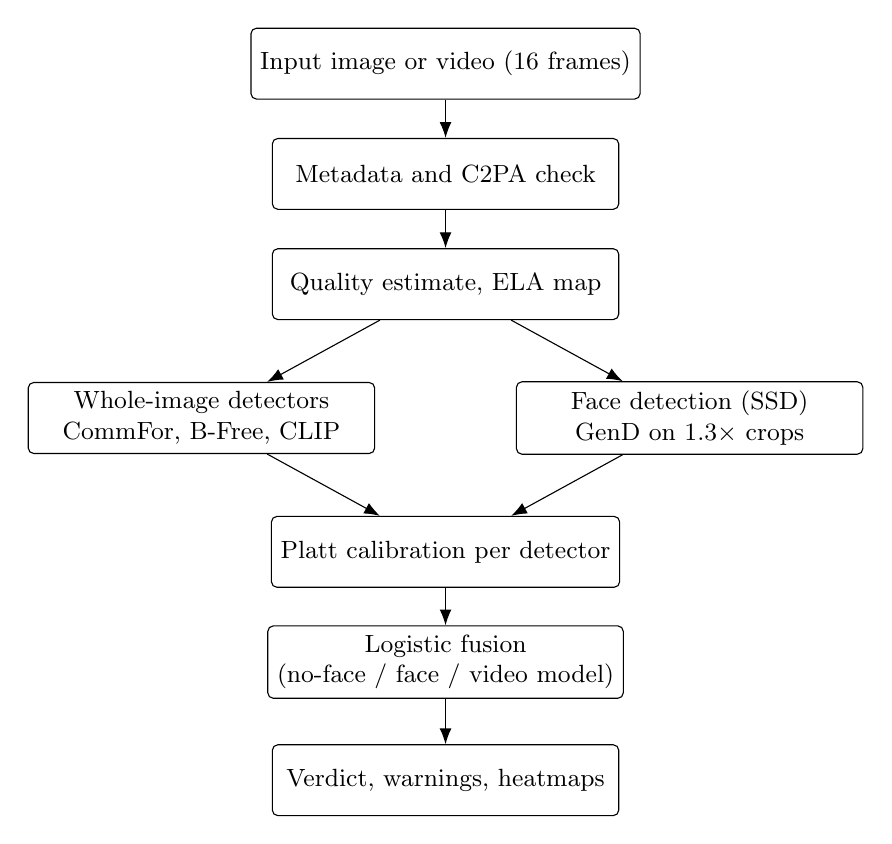
\begin{tikzpicture}[
  box/.style={draw, rounded corners=2pt, align=center, minimum width=44mm, minimum height=9mm, font=\small},
  arr/.style={-{Latex[length=2mm]}}]
\node[box] (in) at (0,0) {Input image or video (16 frames)};
\node[box] (prov) at (0,-1.4) {Metadata and C2PA check};
\node[box] (q) at (0,-2.8) {Quality estimate, ELA map};
\node[box] (pix) at (-3.1,-4.5) {Whole-image detectors\\CommFor, B-Free, CLIP};
\node[box] (face) at (3.1,-4.5) {Face detection (SSD)\\GenD on 1.3$\times$ crops};
\node[box] (cal) at (0,-6.2) {Platt calibration per detector};
\node[box] (fuse) at (0,-7.6) {Logistic fusion\\(no-face / face / video model)};
\node[box] (out) at (0,-9.1) {Verdict, warnings, heatmaps};
\draw[arr] (in) -- (prov);
\draw[arr] (prov) -- (q);
\draw[arr] (q) -- (pix);
\draw[arr] (q) -- (face);
\draw[arr] (pix) -- (cal);
\draw[arr] (face) -- (cal);
\draw[arr] (cal) -- (fuse);
\draw[arr] (fuse) -- (out);
\end{tikzpicture}
\caption{Deepfake forensics pipeline}\label{fig:pipeline}
\end{figure}

\section{Investigation Logic}
The investigation endpoint runs both pipelines on the same file and applies the rules in Table~\ref{tab:verdict}, in order.

\begin{table}[H]
\centering
\caption{Incident verdict rules}\label{tab:verdict}
\begin{tabularx}{\textwidth}{@{}lXl@{}}
\toprule
Condition & Verdict & Threat level \\
\midrule
Fake and weapon seen & Fabricated threat (deepfake disinformation) & CRITICAL \\
Fake, no weapon & Media manipulation detected & HIGH \\
Authentic and weapon seen & Verified physical security incident & CRITICAL \\
Authentic, more than 15 people & Verified crowd surge & ELEVATED \\
Otherwise & Routine capture & SAFE \\
\bottomrule
\end{tabularx}
\end{table}

If the forensics analysis fails, for example on an unreadable file, the endpoint returns an error and does not produce any verdict. An earlier version treated a failure as a score of zero, which would have marked the footage as authentic.

\section{API Design}
\begin{table}[H]
\centering
\caption{Main API endpoints}\label{tab:api}
\begin{tabularx}{\textwidth}{@{}llX@{}}
\toprule
Method & Endpoint & Purpose \\
\midrule
GET & /api/health & GPU memory, loaded models, calibration status \\
POST & /api/crowd/detect & Crowd analysis of one image \\
POST & /api/crowd/video & Crowd analysis of a video with key frames \\
POST & /predict & Deepfake analysis (mode: auto, deepfake, ai\_generated) \\
POST & /api/predict/stream & Same analysis with stage-by-stage progress (SSE) \\
POST & /api/investigate & Combined crowd and forensics verdict \\
POST & /fetch-url & Download media from a URL for analysis \\
POST & /feedback & Store an operator correction \\
\bottomrule
\end{tabularx}
\end{table}

\section{User Interface Design}
The console has four views. \emph{Surveillance} shows annotated frames with counts and risk. \emph{Forensics} shows the verdict, the four model cards, warnings and the evidence heatmaps. \emph{Investigation} shows the combined incident verdict. \emph{Review 2} lists the planned features. A neutral amber style is used when there is no verdict (no face found, or a check could not run), so that such a result is not mistaken for ``authentic''.

% =====================================================================
\chapter{Implementation}
% =====================================================================

\section{Project Structure}
\begin{verbatim}
CrowdGuardAI/
  app.py               FastAPI server, routes, pipeline
  gend_worker.py       face-forensics worker (port 8001)
  crowd/               YOLO detector, tracker, behaviour, risk engine
  detectors/           CommFor, B-Free, CLIP, calibration, fusion,
                       video sampling, ELA/heatmaps, provenance
  data/                calibration.json, eval_scores.json
  tools/               dataset download, calibration, video evaluation
  pretrained_weights/  model weights (not in git)
frontend/              Next.js console (src/components, src/lib/api.ts)
\end{verbatim}

\section{Crowd Module}
\texttt{YOLODetector} wraps the Ultralytics tracker with a generated ByteTrack configuration (high threshold 0.30, low threshold 0.05, new-track threshold 0.30, match threshold 0.80). The person confidence threshold is 0.20 with IoU 0.70, and very small boxes need a slightly higher score. The loader looks for custom weights (\texttt{best.pt}) first and falls back to \texttt{yolo\_crowd.pt}, a YOLOv8n model for the person class. A MobileNetV3-Small weapon classifier (gun and knife) is wired in, but its trained weights are part of the second review, so it is currently inactive. For video, between 6 and 16 frames are sampled depending on the length of the clip.

\section{Whole-Image Detectors}
\textbf{Community Forensics.} The released ViT-S/16 weights are downloaded from Hugging Face (\texttt{OwensLab/commfor-model-384}). The image is resized so its shorter side is 440 pixels, centre-cropped to 384, and scored together with its horizontal flip. The two outputs are averaged.

\textbf{B-Free.} The official code and weights (DINOv2-reg4 ViT-B/14) were taken from the authors' repository. The model scores five 504-pixel crops at native resolution, without resizing, and averages them. To keep memory within 6 GB, images with a side longer than 1024 pixels are centre-cropped (never resized, since resizing removes the traces B-Free looks for), and half precision is used. The wrapper was checked against the four demo images published by the authors, and the logits matched to four decimal places.

\textbf{UniversalFakeDetect.} A frozen CLIP ViT-L/14 with the authors' trained linear layer (\texttt{fc\_weights.pth}) scores a 224-pixel centre crop.

\section{Face Worker}
Faces are found with the OpenCV ResNet-10 SSD detector\cite{bradski2000} at confidence 0.5, with a Haar cascade as fallback. Faces smaller than 40 pixels are ignored. Each face is cropped as a square 1.3 times the size of the detected box, which follows GenD's own preprocessing, and up to three faces per frame are scored. For an image, the score of the most suspicious face is returned. For a video, 16 frames are sampled. The most suspicious face is taken per frame, and the mean of the top half of these frame scores is returned. The worker also reports which model it used and how many frames had a face. If the GenD weights are missing, a generic fallback classifier is loaded, and the result carries a warning.

\section{Calibration and Fusion}
\texttt{tools/calibrate.py} scores every image in the evaluation set with all detectors, using raw (uncalibrated) outputs, and then fits two things on the \emph{fit} half:
\begin{enumerate}
  \item a Platt function $p = \sigma(a \cdot \mathrm{logit}(s) + b)$ for each detector, with class-balanced weights;
  \item a logistic regression on the calibrated logits, $z = b + \sum_i w_i \, \mathrm{logit}(p_i)$, once for images without a scored face (CommFor, B-Free, CLIP) and once for images with one (adding GenD).
\end{enumerate}
The fitted values are written to \texttt{data/calibration.json} and loaded by the live server, so the server applies exactly the logic that was measured. The same file stores the held-out metrics, and \texttt{/api/health} reports whether a fitted calibration is present.

\section{Video Handling}
Sixteen frames are sampled evenly across the clip. For each detector, the per-frame calibrated scores are reduced to one number by taking the mean of the most suspicious half. Version~1 used eight frames and a trimmed mean, which averaged away manipulations that appear in only part of a clip. The per-frame fused scores are also returned, so that the console can show where in the clip the suspicious frames are. \texttt{tools/eval\_video.py} fits a separate video fusion model on Celeb-DF when it is run, and the server picks it up automatically.

\section{Explainability and Provenance}
The response contains an ELA map, a noise residual map and a 24$\times$24 patch map taken from the Community Forensics ViT head. When a face is found, the ratio of ELA error inside the face box to the background is also reported. In version~1 this ratio could override the verdict. It is now shown only as supporting evidence, because JPEG re-compression changes it a lot. If the metadata or a C2PA manifest declares that the file was AI-generated, the final score is raised to at least 0.99.

\section{Error Handling}
The face-worker client returns a structured result with an \texttt{error} field. A missing face score now has two possible meanings: ``no face found'' (a valid answer) or ``check did not run'' (worker down, timeout, or model missing). In Deepfake mode the second case returns \emph{Inconclusive} rather than ``Authentic Face''. In Auto mode the verdict is computed from the whole-image detectors and a warning is shown. The console displays every warning above the score bar.

\section{Web Console}
The frontend is written in TypeScript with Next.js 14. \texttt{src/lib/api.ts} holds typed request functions. These also treat a backend response of \texttt{success:false} as an error, so the views never try to draw a missing result. Sample images and videos are served from \texttt{public/static/samples} so that the test buttons work on a fresh clone.

\screenshot{Surveillance view with person tracking and risk level}{fig:ui-surv}
\screenshot{Forensics view showing the verdict, model scores and heatmaps}{fig:ui-foren}
\screenshot{Investigation view with the combined incident verdict}{fig:ui-inv}

% =====================================================================
\chapter{Evaluation and Results}
% =====================================================================

\section{Problems Found in Version 1}
The first complete version worked end to end, but its deepfake results on new images and videos were poor. Before changing anything, each part was measured separately. The main findings were:
\begin{itemize}
  \item \textbf{The pixel detector produced nearly constant output.} The NPR ResNet-50 file in the project gave logits around $-100$ for almost every image, real or fake. Its AUC on labelled data was about 0.50, which is no better than chance. The file size matched a training checkpoint in the NPR repository, not the released model. The released model also stayed near chance on this data.
  \item \textbf{The face model was not GenD.} The documentation said GenD, but the worker was loading a generic ViT classifier. On the face images in the evaluation set its AUC was 0.58, and it flagged 43\% of real faces as fake.
  \item \textbf{No calibration.} The calibration file contained identity values, so raw scores from different models were compared directly.
  \item \textbf{Hand-set rules.} Weights and thresholds between 0.38 and 0.48 had been chosen by hand. One rule capped the score at 0.36 when two detectors disagreed, which forced some fakes to be labelled real.
  \item \textbf{Silent failure.} If the face worker timed out, Deepfake mode used a face score of 0.0 and reported ``Authentic Face''.
  \item \textbf{Unreliable old benchmark.} The 400-image benchmark file in the project was 82\% fake and its source and labels could not be confirmed, so it was discarded.
\end{itemize}

\section{Evaluation Data}
All evaluation data was downloaded from public sources with their original labels (Table~\ref{tab:data}).

\begin{table}[H]
\centering
\caption{Labelled image data used for calibration and testing}\label{tab:data}
\begin{tabularx}{\textwidth}{@{}Xlr@{}}
\toprule
Source and subset & Label & Images \\
\midrule
Defactify\cite{defactify} validation, MS-COCO photographs & Real & 250 \\
Defactify: SD 2.1, SDXL, SD 3, DALL-E 3, Midjourney & Fake & 5 $\times$ 50 \\
DeepFakeFace\cite{song2023}: IMDB-WIKI faces & Real & 250 \\
DeepFakeFace: InsightFace swap, SD inpainting, SD 1.5 & Fake & 3 $\times$ 83 \\
GenD sample crops: FF++\cite{rossler2019} and Celeb-DF\cite{li2020} & Both & 32 \\
\midrule
Total & 512 real, 519 fake & 1,031 \\
\bottomrule
\end{tabularx}
\end{table}

For video, 189 test videos (100 real, 89 fake) were downloaded from the official Celeb-DF v2 test list.

\section{Protocol}
Every image was scored twice: as downloaded and after re-saving as JPEG at quality 85. The second copy is closer to images shared on messaging apps. This gives 2,062 scored variants. Images were split into a fit half and a test half using the parity of the SHA-1 hash of the file path, and both copies of an image always fall in the same half. All numbers below are on the 1,010 test variants, which were not used for fitting.

Version~1 was replayed on the same test split with its original NPR weights, its original face classifier and its original decision rules. Its compression re-weighting and ELA override were left out of the replay, so the version~1 figures are a close approximation, not an exact copy.

The metrics used are: \emph{fakes detected} (true positive rate), \emph{real correct} (true negative rate), \emph{balanced accuracy} (their mean) and the area under the ROC curve (AUC).

\section{Fitted Calibration}
\begin{table}[H]
\centering
\caption{Fitted Platt coefficients and fusion weights}\label{tab:calib}
\begin{tabular}{@{}lrrrr@{}}
\toprule
Detector & Platt $a$ & Platt $b$ & No-face weight & Face weight \\
\midrule
Community Forensics & 0.550 & 3.471 & 0.660 & 0.616 \\
B-Free & 0.454 & 0.819 & 0.484 & 0.392 \\
UniversalFakeDetect CLIP & 0.290 & 1.927 & 0.479 & 0.224 \\
GenD (face) & 0.713 & $-0.031$ & -- & 1.112 \\
Intercept & & & 0.085 & $-0.427$ \\
\bottomrule
\end{tabular}
\end{table}

The large positive $b$ values for Community Forensics and CLIP mean that their raw scores were much too low on this data. Many fakes had raw scores close to zero. This explains why the fixed thresholds of version~1 missed so many fakes. When a face is present, GenD gets the largest weight, which matches its purpose.

\section{Overall Results}
\begin{table}[H]
\centering
\caption{Held-out results, version 1 and version 2 (percentages)}\label{tab:overall}
\begin{tabular}{@{}lrrrrrrr@{}}
\toprule
& & \multicolumn{3}{c}{Version 1} & \multicolumn{3}{c}{Version 2} \\
\cmidrule(lr){3-5}\cmidrule(lr){6-8}
Group & n & Fake & Real & Bal. & Fake & Real & Bal. \\
\midrule
All test variants & 1010 & 62 & 76 & 69 & 79 & 96 & 88 \\
Original files & 505 & 62 & 75 & 69 & 79 & 96 & 87 \\
JPEG quality 85 & 505 & 63 & 77 & 70 & 80 & 96 & 88 \\
Face scored & 615 & 78 & 55 & 66 & 83 & 94 & 88 \\
No face & 395 & 31 & 100 & 65 & 73 & 99 & 86 \\
\bottomrule
\end{tabular}
\end{table}

The AUC of version~2 is 0.943 overall (0.941 on original files, 0.944 on JPEG copies, 0.954 when a face is scored and 0.924 without a face). Version~1 was a rule system without a single continuous score, so no AUC is given for it. Detection of fakes rose by 17 points while false alarms on real images fell from 24\% to 4\%. The results on original files and JPEG copies are almost the same, so moderate compression does not hurt the new pipeline.

\section{Results by Generator}
\begin{table}[H]
\centering
\caption{Correct decisions by subset (percentages)}\label{tab:subset}
\begin{tabular}{@{}llrrr@{}}
\toprule
Subset & Label & n & Version 1 & Version 2 \\
\midrule
Defactify, MS-COCO & Real & 226 & 95 & 99 \\
Stable Diffusion 2.1 & Fake & 50 & 96 & 100 \\
SDXL & Fake & 52 & 52 & 96 \\
Stable Diffusion 3 & Fake & 42 & 36 & 95 \\
DALL-E 3 & Fake & 62 & 13 & 40 \\
Midjourney & Fake & 48 & 4 & 65 \\
DeepFakeFace, IMDB-WIKI & Real & 222 & 57 & 97 \\
InsightFace swap & Fake & 98 & 55 & 46 \\
SD inpainting & Fake & 96 & 99 & 100 \\
SD 1.5 text-to-image & Fake & 86 & 100 & 100 \\
\bottomrule
\end{tabular}
\end{table}

\begin{figure}[H]
\centering
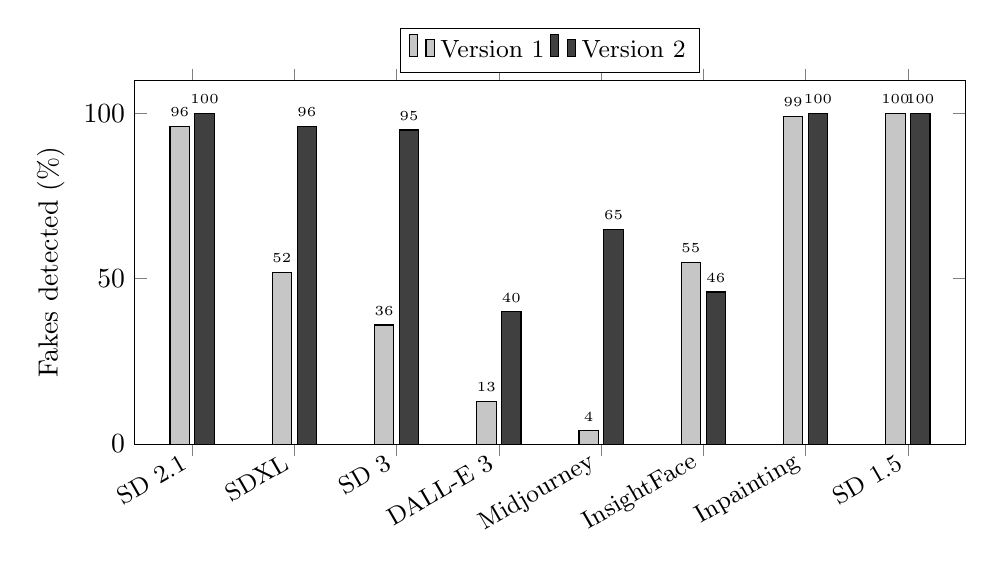
\begin{tikzpicture}
\begin{axis}[ybar, bar width=7pt, width=\textwidth, height=6.2cm,
  ymin=0, ymax=110, ylabel={Fakes detected (\%)},
  symbolic x coords={a,b,c,d,e,f,g,h}, xtick=data,
  xticklabels={SD 2.1,SDXL,SD 3,DALL-E 3,Midjourney,InsightFace,Inpainting,SD 1.5},
  x tick label style={rotate=30,anchor=east,font=\small},
  legend style={at={(0.5,1.02)},anchor=south,legend columns=2,font=\small},
  nodes near coords, nodes near coords style={font=\tiny}, enlarge x limits=0.08]
\addplot[fill=gray!45] coordinates {(a,96) (b,52) (c,36) (d,13) (e,4) (f,55) (g,99) (h,100)};
\addplot[fill=black!75] coordinates {(a,100) (b,96) (c,95) (d,40) (e,65) (f,46) (g,100) (h,100)};
\legend{Version 1, Version 2}
\end{axis}
\end{tikzpicture}
\caption{Fake detection rate by generator, version 1 and version 2}\label{fig:subset}
\end{figure}

The largest gains are on SDXL, Stable Diffusion 3 and Midjourney. Midjourney went from 4\% to 65\%. On real faces the error rate fell from 43\% to 3\%, which was the most visible problem for users of version~1.

InsightFace swaps are the one subset that got worse (55\% to 46\%). The version~1 face classifier flagged a large share of all faces, real or fake, so its 55\% on swaps came together with 43\% false alarms on real faces. Version~2 makes far fewer mistakes overall, but face swaps on small, low-resolution IMDB-WIKI photographs are still hard for GenD. DALL-E 3 remains the weakest generator at 40\%.

On the 28 GenD sample crops (FF++ and Celeb-DF), version~2 detected 86\% of fakes but accepted only 36\% of the real crops. This subset is too small to draw firm conclusions. Its pre-cropped faces also differ from full photographs, and Chapter~6 returns to this point.

\section{Individual Detectors}
\begin{table}[H]
\centering
\caption{Single detectors on the test split (calibrated, threshold 0.5)}\label{tab:single}
\begin{tabular}{@{}lrrrr@{}}
\toprule
Detector & n & AUC & Fake (\%) & Real (\%) \\
\midrule
Community Forensics & 1010 & 0.887 & 76 & 92 \\
B-Free & 1010 & 0.866 & 73 & 90 \\
UniversalFakeDetect CLIP & 1010 & 0.692 & 59 & 68 \\
GenD (faces only) & 615 & 0.828 & 67 & 87 \\
\midrule
NPR, version 1 & 1010 & $\approx$0.50 & -- & -- \\
Generic face ViT, version 1 & 615 & 0.582 & 66 & 51 \\
\bottomrule
\end{tabular}
\end{table}

No single detector reaches the fused result (AUC 0.943). Community Forensics is the strongest model alone. B-Free is close behind and has replaced NPR, which carried no information. CLIP is weak alone, but it still gets a useful fusion weight because its errors differ from those of the other two.

\section{Running Time}
After warm-up, typical GPU times per image were about 0.03~s for Community Forensics, 0.25 to 0.35~s for B-Free, 0.06~s for CLIP, and 0.02 to 0.6~s for face detection with GenD, depending on the number and size of faces. A full image analysis with ELA and heatmaps takes well under two seconds. With all models loaded in one process, GPU memory use was between 4.2 and 4.6~GB of the 6~GB available.

\section{Manual Testing}
After the update, the web console was tested by hand with the sample files supplied with the project and with additional images and videos. The verdicts matched expectations on these files. Table~\ref{tab:manual} records the individual cases.

\begin{table}[H]
\centering
\caption{Manual test cases (to be completed with observed outputs)}\label{tab:manual}
\begin{tabularx}{\textwidth}{@{}lllX@{}}
\toprule
File & Mode & Expected & Observed verdict and score \\
\midrule
F.png & Investigation & Manipulated & \\
R.jpg & Investigation & Authentic & \\
deepfake\_face.jpg & Deepfake & Fake & \\
authentic.jpg & Auto & Real & \\
sample\_diffusion.jpg & AI-Generated & Fake & \\
sample\_deepfake\_video.mp4 & Auto & Fake & \\
surveillance\_sample.mp4 & Surveillance & Crowd counted & \\
\bottomrule
\end{tabularx}
\end{table}

\section{Discussion and Limitations}
The main lesson is that the poor results of version~1 came from the integration, not from the published detectors themselves. One detector carried no information, one model was not the model described in the documentation, and hand-set thresholds sat in the wrong place for raw scores. Measuring each part on labelled data found all of these problems within a day. Guessing would have taken much longer.

The limitations are:
\begin{itemize}
  \item Video results are not yet measured. The Celeb-DF test videos are prepared, but the evaluation run was not completed in time.
  \item The calibration data comes from five commercial and open generators and two face datasets. Newer generators such as Flux, or heavy social-media compression, may behave differently.
  \item DALL-E 3 images and InsightFace swaps are still detected less than half the time.
  \item The weapon classifier is not trained yet, so weapon-based verdicts depend only on what the YOLO model detects.
  \item B-Free's licence allows only non-profit use, which matters if the system is ever deployed commercially.
\end{itemize}

% =====================================================================
\chapter{Conclusions}
% =====================================================================

\section{Conclusions}
CrowdGuard AI joins crowd monitoring and media forensics in one tool, and the combined verdict separates real incidents from fabricated footage. The main technical result of this report is the rebuilt deepfake module. Published detectors were wired in correctly, and their scores were calibrated and fused with weights fitted on public labelled data. Measured on images the module had never seen, balanced accuracy rose from 69\% to 88\% (AUC 0.943), and false alarms on real faces fell from 43\% to 3\%. The system also states clearly when a check did not run. In version~1, a failed check could be reported as authentic.

\section{Future Work}
\begin{enumerate}
  \item Run \texttt{tools/eval\_video.py} on the 189 Celeb-DF test videos, fit the video fusion model and report video accuracy.
  \item Add recent generators (Flux, SD 3.5) and images re-shared through messaging apps to the calibration set, and look at DALL-E 3 and face-swap failures in particular.
  \item Train the weapon detector and classifier (second review).
  \item Add optical-flow crowd motion analysis and live RTSP streams from several cameras.
  \item Generate signed PDF incident reports and store incidents in a database.
  \item Use operator feedback, collected through \texttt{/feedback}, for periodic recalibration.
\end{enumerate}

% =====================================================================
\begin{thebibliography}{99}
\addcontentsline{toc}{chapter}{Bibliography and References}
\setlength{\itemsep}{2pt}

\bibitem{goodfellow2014} Goodfellow I, Pouget-Abadie J, Mirza M, Xu B, Warde-Farley D, Ozair S, Courville A and Bengio Y, ``Generative adversarial nets.'' Advances in Neural Information Processing Systems. 2014, 27, 2672--2680.

\bibitem{ho2020} Ho J, Jain A and Abbeel P, ``Denoising diffusion probabilistic models.'' Advances in Neural Information Processing Systems. 2020, 33, 6840--6851.

\bibitem{rombach2022} Rombach R, Blattmann A, Lorenz D, Esser P and Ommer B, ``High-resolution image synthesis with latent diffusion models.'' IEEE/CVF Conference on Computer Vision and Pattern Recognition. 2022, 10684--10695.

\bibitem{tolosana2020} Tolosana R, Vera-Rodriguez R, Fierrez J, Morales A and Ortega-Garcia J, ``Deepfakes and beyond: A survey of face manipulation and fake detection.'' Information Fusion. 2020, 64, 131--148.

\bibitem{wang2020} Wang SY, Wang O, Zhang R, Owens A and Efros AA, ``CNN-generated images are surprisingly easy to spot... for now.'' IEEE/CVF Conference on Computer Vision and Pattern Recognition. 2020, 8695--8704.

\bibitem{ojha2023} Ojha U, Li Y and Lee YJ, ``Towards universal fake image detectors that generalize across generative models.'' IEEE/CVF Conference on Computer Vision and Pattern Recognition. 2023, 24480--24489.

\bibitem{radford2021} Radford A, Kim JW, Hallacy C, et al., ``Learning transferable visual models from natural language supervision.'' International Conference on Machine Learning. 2021, PMLR 139, 8748--8763.

\bibitem{tan2024} Tan C, Zhao Y, Wei S, Gu G, Liu P and Wei Y, ``Rethinking the up-sampling operations in CNN-based generative network for generalizable deepfake detection.'' IEEE/CVF Conference on Computer Vision and Pattern Recognition. 2024, 28130--28139.

\bibitem{park2025} Park J and Owens A, ``Community Forensics: Using thousands of generators to train fake image detectors.'' IEEE/CVF Conference on Computer Vision and Pattern Recognition. 2025.

\bibitem{dosovitskiy2021} Dosovitskiy A, Beyer L, Kolesnikov A, et al., ``An image is worth 16x16 words: Transformers for image recognition at scale.'' International Conference on Learning Representations. 2021.

\bibitem{guillaro2025} Guillaro F, Zingarini G, Usman B, Sud A, Cozzolino D and Verdoliva L, ``A bias-free training paradigm for more general AI-generated image detection.'' IEEE/CVF Conference on Computer Vision and Pattern Recognition. 2025, 18685--18694.

\bibitem{oquab2024} Oquab M, Darcet T, Moutakanni T, et al., ``DINOv2: Learning robust visual features without supervision.'' Transactions on Machine Learning Research. 2024.

\bibitem{darcet2024} Darcet T, Oquab M, Mairal J and Bojanowski P, ``Vision transformers need registers.'' International Conference on Learning Representations. 2024.

\bibitem{rossler2019} R\"ossler A, Cozzolino D, Verdoliva L, Riess C, Thies J and Nie{\ss}ner M, ``FaceForensics++: Learning to detect manipulated facial images.'' IEEE/CVF International Conference on Computer Vision. 2019, 1--11.

\bibitem{li2020} Li Y, Yang X, Sun P, Qi H and Lyu S, ``Celeb-DF: A large-scale challenging dataset for DeepFake forensics.'' IEEE/CVF Conference on Computer Vision and Pattern Recognition. 2020, 3207--3216.

\bibitem{yermakov2026} Yermakov A, Cech J, Matas J and Fritz M, ``Deepfake detection that generalizes across benchmarks.'' IEEE/CVF Winter Conference on Applications of Computer Vision. 2026, 773--783.

\bibitem{song2023} Song H, Huang S, Dong Y and Tu WW, ``Robustness and generalizability of deepfake detection: A study with diffusion models.'' arXiv preprint arXiv:2309.02218. 2023.

\bibitem{guo2017} Guo C, Pleiss G, Sun Y and Weinberger KQ, ``On calibration of modern neural networks.'' International Conference on Machine Learning. 2017, PMLR 70, 1321--1330.

\bibitem{platt1999} Platt J. In Advances in Large Margin Classifiers, ``Probabilistic outputs for support vector machines and comparisons to regularized likelihood methods''; MIT Press, Cambridge, 1999, pp 61--74.

\bibitem{jocher2023} Jocher G, Chaurasia A and Qiu J, ``Ultralytics YOLOv8'', 2023, https://github.com/ultralytics/ultralytics

\bibitem{zhang2022} Zhang Y, Sun P, Jiang Y, et al., ``ByteTrack: Multi-object tracking by associating every detection box.'' European Conference on Computer Vision. 2022, 1--21.

\bibitem{howard2019} Howard A, Sandler M, Chu G, et al., ``Searching for MobileNetV3.'' IEEE/CVF International Conference on Computer Vision. 2019, 1314--1324.

\bibitem{krawetz2007} Krawetz N, ``A picture's worth: Digital image analysis and forensics.'' Black Hat Briefings, USA, 2007.

\bibitem{c2pa} Coalition for Content Provenance and Authenticity, ``C2PA Technical Specification'', https://c2pa.org/specifications/

\bibitem{fastapi} Ram\'irez S, ``FastAPI'', https://fastapi.tiangolo.com

\bibitem{nextjs} Vercel, ``Next.js Documentation'', https://nextjs.org/docs

\bibitem{bradski2000} Bradski G, ``The OpenCV Library.'' Dr. Dobb's Journal of Software Tools. 2000.

\bibitem{defactify} Roy R, et al., ``Defactify Image Dataset'', Hugging Face, https://huggingface.co/datasets/Rajarshi-Roy-research/Defactify\_Image\_Dataset

\end{thebibliography}

% =====================================================================
\appendix
\chapter{List of Abbreviations}
\begin{tabular}{@{}ll@{}}
AUC & Area Under the ROC Curve \\
API & Application Programming Interface \\
C2PA & Coalition for Content Provenance and Authenticity \\
CCTV & Closed-Circuit Television \\
CLIP & Contrastive Language-Image Pre-training \\
CUDA & Compute Unified Device Architecture \\
DFF & DeepFakeFace dataset \\
ELA & Error Level Analysis \\
FF++ & FaceForensics++ \\
GAN & Generative Adversarial Network \\
GPU & Graphics Processing Unit \\
IoU & Intersection over Union \\
NPR & Neighboring Pixel Relationships \\
ROC & Receiver Operating Characteristic \\
SD & Stable Diffusion \\
SSE & Server-Sent Events \\
SSD & Single Shot Detector \\
ViT & Vision Transformer \\
YOLO & You Only Look Once \\
\end{tabular}

\chapter{Setup and Reproduction}
\textbf{Model weights} (not stored in git), placed in \texttt{CrowdGuardAI/pretrained\_weights/}: \texttt{yolo\_crowd.pt}, \texttt{fc\_weights.pth}, and the folder \texttt{GenD/} (from \texttt{yermandy/GenD\_CLIP\_L\_14}). B-Free weights go in \texttt{CrowdGuardAI/detectors/B-Free/code/weights/BFREE\_dino2reg4/}. Community Forensics and the face detector files are downloaded automatically on first run.

\textbf{Running the system}
\begin{verbatim}
cd frontend
npm install
npm run build
cd ..
run_crowdguard.bat
\end{verbatim}

\textbf{Reproducing the evaluation}
\begin{verbatim}
cd CrowdGuardAI
..\venv_gend\Scripts\python.exe tools\build_eval_set.py
..\venv_gend\Scripts\python.exe tools\calibrate.py
..\venv_gend\Scripts\python.exe tools\build_video_eval.py
..\venv_gend\Scripts\python.exe tools\eval_video.py
\end{verbatim}

The first two commands download the labelled images and write \texttt{data/calibration.json} together with the held-out metrics reported in Chapter~5. The last two prepare and evaluate the Celeb-DF test videos.

% ================= PLAGIARISM VERIFICATION =================
\clearpage
\begin{center}\textbf{PLAGIARISM VERIFICATION}\\(This certificate has to be attached at the backside of the dissertation)\end{center}

Title of the dissertation: CrowdGuard AI: An Integrated System for Crowd Threat Monitoring and Deepfake Media Verification

This is to report that the above thesis was scanned for similarity detection. Process and outcome is given below:

\textbf{Software used} \dotfill \textbf{Date} \dotfill

\textbf{Similarity Index} \dotfill \textbf{Total word count} \dotfill

The complete report is submitted for review by the Supervisor/Co-supervisor.

\vspace{1cm}
Checked by Name \& Signature \hfill \textbf{Library Head Name \& Sign}

\vspace{0.8cm}
The complete report of the above thesis has been reviewed by the undersigned. (Check Box)

$\square$ The similarity index is below accepted norms.

$\square$ The similarity index is above accepted norms, because of the following reasons:

\dotfill\\ \dotfill\\ \dotfill

$\square$ The dissertation may be considered for the award of degree. (Relevant documents attached).

\vspace{1.5cm}
\begin{tabular}{@{}p{0.31\textwidth}p{0.31\textwidth}p{0.31\textwidth}@{}}
\textbf{Name \& Sign of Student} & \textbf{Name \& Sign of Supervisor} & \textbf{Name \& Sign of Co-Supervisor}
\end{tabular}

\end{document}
